\section{Experimental Results}
\label{sec:experiments}

We evaluate motion generation as a foundation for humanoid control through benchmark and real-world experiments (Secs.~\ref{sec:exp_simulation}--\ref{sec:exp_real}), followed by analyses of motion priors, scaling, and adaptation design (Secs.~\ref{sec:exp_t2m}--\ref{sec:exp_ablation}). Unless explicitly ablated, all Kimodo-Policy variants retain the pretrained motion backbone. Kimodo-Policy denotes direct downstream fine-tuning, while Kimodo-Policy$^{*}$ additionally initializes the conditioning modules and hand head through policy pretraining on 419 hours of robot-interaction data.

\subsection{Evaluation on the HumanoidArena Benchmark}
\label{sec:exp_simulation}

HumanoidArena~\citep{humanoidarena} comprises seven language-conditioned tasks spanning human--object interaction (HOI) and human--scene interaction (HSI), with substantial requirements for locomotion, posture adjustment, and manipulation (Fig.~\ref{fig:humanoidarena}). We evaluate both independent task-specific policies and a single policy jointly trained on all seven tasks. Success rate (SR) measures task completion, while average fall rate (AFR) characterizes execution stability within the SONIC-based control stack~\citep{sonic}. Real-time chunking (RTC) is disabled in our simulation evaluations.

\begin{figure}[H]
  \centering
  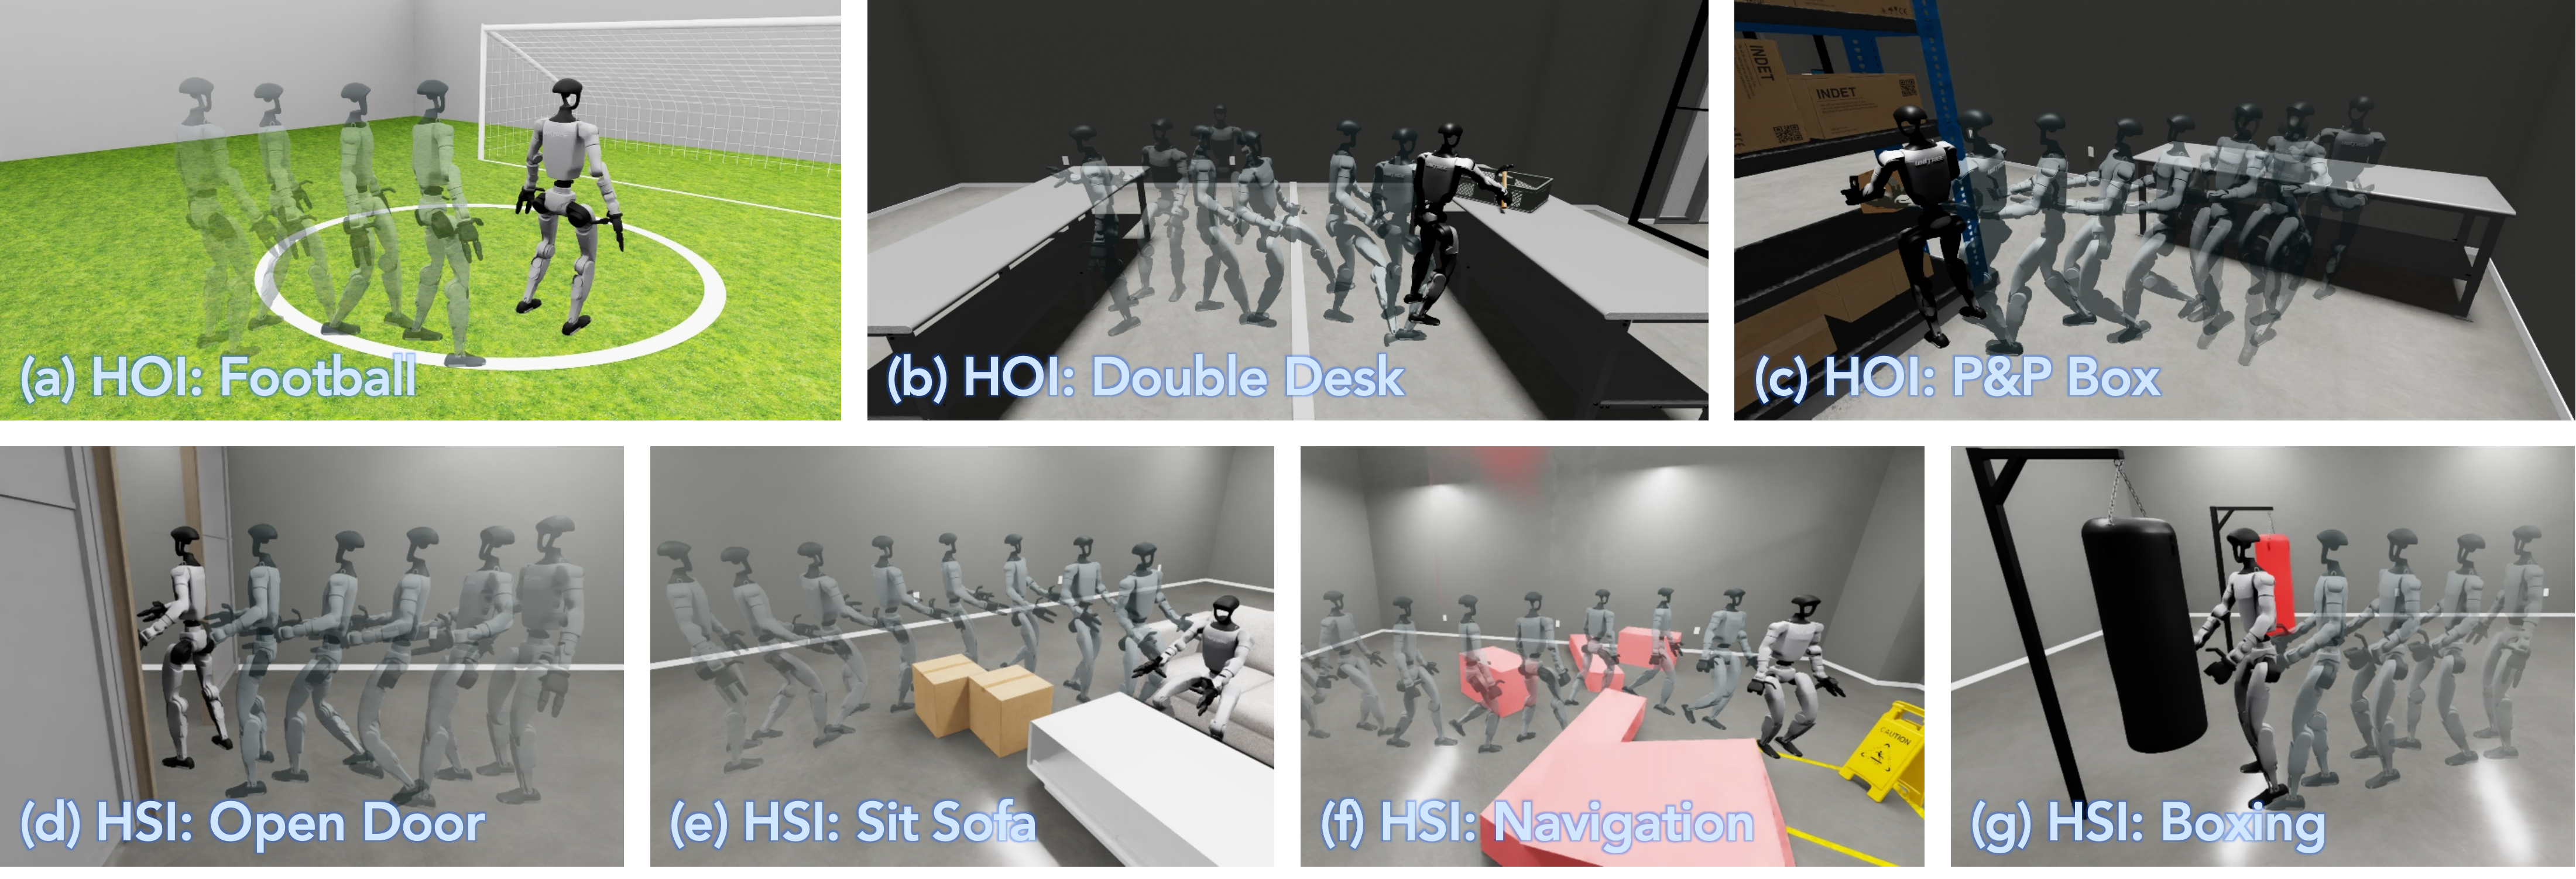
\includegraphics[width=\textwidth]{image/arena.png}
  \caption{\textbf{Visualization of the Seven HumanoidArena Tasks.} The benchmark includes Football, DoubleDesk, P\&Pbox, OpenDoor, SitSofa, Boxing, and VisNavi, covering language-conditioned humanoid behavior across human--object and human--scene interaction with coordinated locomotion, balance, and manipulation.}
  \label{fig:humanoidarena}
\end{figure}

\textbf{Single-task results.} Table~\ref{tab:arena_single_task} shows that Kimodo-Policy achieves the highest overall SR of 69.51\%, exceeding Diffusion Policy (DP)~\citep{chi2023diffusionpolicy}, the strongest baseline in this setting, by 9.51 percentage points. Both Kimodo-Policy variants obtain an AFR of 4.29\%, the lowest reported in the table. The aggregate advantage is concentrated in HSI: direct fine-tuning achieves an HSI average of 84.58\%, compared with 65.83\% for DP, including 100.0\% on SitSofa and 75.0\% on VisNavi. In contrast, its HOI average of 49.44\% remains below DP's 52.22\%. Thus, the motion-based policy is particularly effective on the evaluated scene-interaction tasks, while its advantages do not extend uniformly to every interaction category. Additional policy pretraining yields 67.14\% overall SR, below the 69.51\% obtained by direct fine-tuning. It improves OpenDoor from 90.0\% to 93.3\% and VisNavi from 75.0\% to 76.7\%, but reduces performance on the remaining tasks. These results show that the pretrained motion backbone can support effective task-specific adaptation without the additional robot-interaction pretraining stage; they also indicate that the benefit of that stage depends on the downstream training setting. These scene-interaction tasks require coordinated changes in posture and global position, making the strong HSI performance and low AFR consistent with transferring useful whole-body movement structure.




  




\begin{table}[H]
  \caption{
    \textbf{\textit{Single-task training results on HumanoidArena.}} Each policy is fine-tuned independently on one task. Values are mean $\pm$ standard deviation; $^{*}$ denotes VLA-pretrained initialization. Bold and underlined entries indicate the best and second-best results, respectively.
  }
  \label{tab:arena_single_task}
  \centering
  \arrayrulecolor{hclblue}
  \begin{adjustbox}{max width=\textwidth}
  \setlength{\tabcolsep}{4.2pt}
  \renewcommand{\arraystretch}{1.08}

  \begin{tabular}{cccccc|cccccc}
  \toprule
  & &
  \multicolumn{4}{c|}{\textbf{Human--Object Interaction}} &
  \multicolumn{5}{c}{\textbf{Human--Scene Interaction}} & \\
  \cmidrule(lr){3-6}
  \cmidrule(lr){7-11}

  \multirow{-2}{*}{\textbf{Method}} &
  \multirow{-2}{*}{\textbf{AFR~($\downarrow$)}} &
  \textbf{\textsc{Football}} &
  \textbf{\textsc{DoubleDesk}} &
  \textbf{\textsc{P\&Pbox}} &
  \textbf{\textsc{Avg~($\uparrow$)}} &
  \textbf{\textsc{OpenDoor}} &
  \textbf{\textsc{SitSofa}} &
  \textbf{\textsc{Boxing}} &
  \textbf{\textsc{VisNavi}} &
  \textbf{\textsc{Avg~($\uparrow$)}} &
  \multirow{-2}{*}{\textbf{\textsc{Overall~($\uparrow$)}}} \\
  
  \midrule
  ACT~\cite{ACT}
  & 8.57\%
  & 16.7$\pm$6.2\%
  & 18.3$\pm$4.7\%
  & 56.7$\pm$6.2\%
  & 30.56$\pm$19.36\%
  & 78.3$\pm$9.4\%
  & 73.3$\pm$8.5\%
  & 56.7$\pm$6.2\%
  & 33.3$\pm$2.4\%
  & 60.42$\pm$18.98\%   & 47.61\% \\

  DP~\cite{chi2023diffusionpolicy}
  & 8.33\%
  & \textbf{45.0$\pm$10.8\%}
  & 36.7$\pm$4.7\%
  & 75.0$\pm$4.1\%
  & \textbf{52.22$\pm$17.97\%}
  & 85.0$\pm$10.8\%
  & 78.3$\pm$14.3\%
  & \textbf{76.7$\pm$2.4\%}
  & 23.3$\pm$6.2\%
  & 65.83$\pm$26.52\%   & 60\% \\

  FM~\cite{FM_objective}
  & 5.71\%
  & 13.3$\pm$2.4\%
  & 38.3$\pm$4.7\%
  & 73.3$\pm$6.2\%
  & 41.67$\pm$25.06\%
  & 70.0$\pm$4.1\%
  & 15.0$\pm$14.7\%
  & 70.0$\pm$8.2\%
  & 38.3$\pm$14.3\%
  & 48.33$\pm$26.94\%   & 45.46\% \\

  $\pi_{0.5}$~\cite{pi05}
  & \underline{5.24\%}
  & 10.0$\pm$4.1\%
  & \textbf{43.3$\pm$6.2\%}
  & 71.7$\pm$11.8\%
  & 41.67$\pm$26.46\%
  & 66.7$\pm$6.2\%
  & 73.3$\pm$2.4\%
  & 70.0$\pm$0.0\%
  & 23.3$\pm$6.2\%
  & 58.33$\pm$20.85\%   & 51.19\% \\

  \rowcolor{hclbrown!8!white}
  \texttt{Ours}
  & \textbf{4.29\%}
  & \underline{28.3$\pm$6.2\%}
  & \underline{40.0$\pm$0.0\%}
  & \textbf{80.0$\pm$4.1\%}
  & \underline{49.44$\pm$22.54\%}
  & \underline{90.0$\pm$4.1\%}
  & \textbf{100.0$\pm$0.0\%}
  & \underline{73.3$\pm$13.1\%}
  & \underline{75.0$\pm$10.8\%}
  & \textbf{84.58$\pm$14.06\%}   & \textbf{69.51\%} \\


  \rowcolor{hclbrown!15!white}
  \texttt{Ours}$^{*}$
  & \textbf{4.29\%}
  & 26.7$\pm$4.7\%
  & 28.3$\pm$2.4\%
  & \underline{78.3$\pm$8.5\%}
  & 44.44$\pm$24.66\%
  & \textbf{93.3$\pm$2.4\%}
  & \underline{96.7$\pm$2.4\%}
  & 70.0$\pm$8.2\%
  & \textbf{76.7$\pm$18.9\%}
  & \underline{84.17$\pm$15.25\%}   & \underline{67.14\%} \\

  \bottomrule
  \end{tabular}
  \end{adjustbox}
\end{table}


\textbf{Multi-task results.} Table~\ref{tab:arena_multi_task} extends the comparison to a shared seven-task policy and includes additional VLA and WAM baselines. Kimodo-Policy$^{*}$ achieves the highest overall SR among the compared methods at 72.14\%, exceeding GR00T N1.7 (69.70\%) and GigaWorld-Policy (68.39\%). The gain over GR00T N1.7, the strongest baseline in the table, is 2.44 percentage points. Its AFR is approximately 4.3\%, the lowest among methods for which this metric is reported; AFR is unavailable for several of the added baselines. The task breakdown clarifies the source of this aggregate advantage. Kimodo-Policy$^{*}$ achieves the highest HSI average, approximately 84.2\%, and leads on P\&Pbox and VisNavi while matching HuGe-GR00T on OpenDoor and the directly fine-tuned Kimodo-Policy on SitSofa. Its HOI average, approximately 56.1\%, is below GR00T N1.7's 62.22\% and GigaWorld-Policy's 60.14\%. In particular, Football and DoubleDesk remain challenging relative to the strongest task-specific competitors. The results therefore support the effectiveness of this KAM instantiation across a diverse task set, with its strongest aggregate advantage in scene interaction. Within our framework, policy pretraining increases overall multi-task SR from 67.63\% to 72.14\%, a gain of 4.51 percentage points, with improvements on five tasks, unchanged performance on SitSofa, and a decrease on DoubleDesk. Its benefit in joint training contrasts with the single-task results, suggesting that interaction pretraining is more useful when one set of conditioning modules must support multiple behaviors.

\begin{table}[H]
  \caption{
    \textbf{\textit{Multi-task results on HumanoidArena.}}
    Each policy is trained jointly on the seven benchmark tasks.
    ACT, DP, FM, and $\pi_{0.5}$ results are taken from the official HumanoidArena report~\citep{humanoidarena}. HuGe results are from Table~4 of \citet{liu2026huge}. Entries marked $^{\dagger}$ are from Table~1 of \citet{li2026languageforcing}, with HOI and HSI means computed from the reported task scores.
    $^{*}$ indicates additional policy pretraining, with data and procedures specific to each method. We show mean $\pm$ standard deviation where available and use a dash for unreported values. Bold and underlined entries indicate the best and second-best results, respectively.
   Baselines include ACT~\citep{ACT}, DP~\citep{chi2023diffusionpolicy}, FM~\citep{FM_objective}, $\pi_{0.5}$~\citep{pi05}, HuGe variants~\citep{liu2026huge}, Fast-WAM~\citep{yuan2026fastwam}, LingBot-VA~\citep{li2026lingbotva}, GR00T N1.7~\citep{grootn1}, GigaWorld-Policy~\citep{gigaworld2026policy05}.
  }
  \label{tab:arena_multi_task}
  \centering
  \arrayrulecolor{hclblue}
  \begin{adjustbox}{max width=\textwidth}
  \setlength{\tabcolsep}{4.2pt}
  \renewcommand{\arraystretch}{1.08}

  \begin{tabular}{cccccc|cccccc}
  \toprule
  & &
  \multicolumn{4}{c|}{\textbf{Human--Object Interaction}} &
  \multicolumn{5}{c}{\textbf{Human--Scene Interaction}} & \\
  \cmidrule(lr){3-6}
  \cmidrule(lr){7-11}

  \multirow{-2}{*}{\textbf{Method}} &
  \multirow{-2}{*}{\textbf{AFR~($\downarrow$)}} &
  \textbf{\textsc{Football}} &
  \textbf{\textsc{DoubleDesk}} &
  \textbf{\textsc{P\&Pbox}} &
  \textbf{\textsc{Avg~($\uparrow$)}} &
  \textbf{\textsc{OpenDoor}} &
  \textbf{\textsc{SitSofa}} &
  \textbf{\textsc{Boxing}} &
  \textbf{\textsc{VisNavi}} &
  \textbf{\textsc{Avg~($\uparrow$)}} &
  \multirow{-2}{*}{\textbf{\textsc{Overall~($\uparrow$)}}} \\
  \midrule

  ACT
  & 7.4\%
  & 20.0$\pm$4.1\%
  & 30.0$\pm$4.1\%
  & 60.0$\pm$12.2\%
  & 36.7$\pm$18.7\%
  & 58.3$\pm$2.4\%
  & 21.7$\pm$2.4\%
  & 58.3$\pm$10.3\%
  & 28.3$\pm$4.7\%
  & 41.7$\pm$17.8\%
  & 39.5\% \\

  DP
  & 7.1\%
  & 53.3$\pm$6.2\%
  & 35.0$\pm$10.8\%
  & 0.0$\pm$0.0\%
  & 29.4$\pm$23.3\%
  & 83.3$\pm$6.2\%
  & \underline{83.3$\pm$4.7\%}
  & 21.7$\pm$30.6\%
  & 50.0$\pm$14.7\%
  & 59.6$\pm$31.1\%
  & 46.7\% \\

  FM
  & 7.1\%
  & 21.7$\pm$8.5\%
  & 20.0$\pm$7.1\%
  & 0.0$\pm$0.0\%
  & 13.9$\pm$11.7\%
  & 76.7$\pm$2.4\%
  & 48.3$\pm$6.2\%
  & 18.3$\pm$25.9\%
  & 38.3$\pm$6.2\%
  & 45.4$\pm$25.1\%
  & 31.9\% \\

  $\pi_{0.5}$
  & 6.4\%
  & 10.0$\pm$7.1\%
  & 30.0$\pm$7.1\%
  & 75.0$\pm$4.1\%
  & 38.3$\pm$27.9\%
  & 85.0$\pm$4.1\%
  & 70.0$\pm$14.7\%
  & 71.7$\pm$12.5\%
  & 35.0$\pm$4.1\%
  & 65.4$\pm$21.1\%
  & 53.8\% \\

  HuGe-OFT$^{*}$
  & ---
  & 48.33\%
  & 0.00\%
  & 53.33\%
  & 33.89\%
  & 75.00\%
  & 55.00\%
  & \underline{73.33\%}
  & \underline{73.33\%}
  & 69.17\%
  & 54.05\% \\

  HuGe-GR00T$^{*}$
  & ---
  & \textbf{71.67\%}
  & 15.00\%
  & \underline{81.67\%}
  & 56.11\%
  & \textbf{95.00\%}
  & 78.33\%
  & 68.33\%
  & 56.67\%
  & 74.58\%
  & 66.67\% \\

  HuGe-Pi$^{*}$
  & ---
  & 63.33\%
  & 11.67\%
  & 76.67\%
  & 50.56\%
  & 88.33\%
  & \underline{83.33\%}
  & 68.33\%
  & 63.33\%
  & 75.83\%
  & 65.00\% \\

  Fast-WAM$^{\dagger}$
  & ---
  & 46.25\%
  & 45.00\%
  & 73.75\%
  & 55.00\%
  & 85.42\%
  & 74.58\%
  & 67.92\%
  & 35.00\%
  & 65.73\%
  & 61.13\% \\

  LingBot-VA$^{\dagger}$
  & ---
  & 51.67\%
  & 41.25\%
  & 77.92\%
  & 56.95\%
  & 84.58\%
  & 77.08\%
  & 72.92\%
  & 52.08\%
  & 71.67\%
  & 65.36\% \\

  GR00T N1.7$^{\dagger}$
  & ---
  & \underline{63.75\%}
  & \underline{49.58\%}
  & 73.33\%
  & \textbf{62.22\%}
  & 82.08\%
  & 76.67\%
  & \textbf{76.67\%}
  & 65.83\%
  & 75.31\%
  & \underline{69.70\%} \\

  GigaWorld-Policy$^{\dagger}$
  & ---
  & 62.08\%
  & \textbf{52.50\%}
  & 65.83\%
  & \underline{60.14\%}
  & 90.83\%
  & 74.17\%
  & \underline{73.33\%}
  & 60.00\%
  & 74.58\%
  & 68.39\% \\

  \rowcolor{hclbrown!8!white}
  \texttt{Ours}
  & \underline{5.0\%}
  & 35.0$\pm$7.1\%
  & 40.0$\pm$0.0\%
  & 80.0$\pm$4.1\%
  & 51.7$\pm$20.7\%
  & \underline{93.3$\pm$6.2\%}
  & \textbf{96.7$\pm$4.7\%}
  & 66.7$\pm$4.7\%
  & 61.7$\pm$6.2\%
  & \underline{79.6$\pm$16.5\%}
  & 67.6\% \\

  \rowcolor{hclbrown!15!white}
  \texttt{Ours}$^{*}$
  & \textbf{4.3\%}
  & 40.0$\pm$4.1\%
  & 38.3$\pm$2.4\%
  & \textbf{90.0$\pm$4.1\%}
  & 56.1$\pm$24.2\%
  & \textbf{95.0$\pm$4.1\%}
  & \textbf{96.7$\pm$4.7\%}
  & 68.3$\pm$10.3\%
  & \textbf{76.7$\pm$8.5\%}
  & \textbf{84.2$\pm$14.1\%}
  & \textbf{72.1\%} \\

  \bottomrule
  \end{tabular}
  \end{adjustbox}
\end{table}


\textbf{Qualitative visual grounding.} Figure~\ref{fig:attention} visualizes responses around task-relevant objects and interaction regions, including the ball, box, and punching bag. In the displayed examples, Kimodo-Policy exhibits localized responses near these regions, whereas DP often produces more spatially diffuse activation. This pattern is consistent with the intended role of perception in a KAM: visual observations condition where the inherited movement patterns should be expressed. These maps provide qualitative context for the control results, but do not establish causal feature importance or instruction sensitivity, since the examples also differ in scene content.

\begin{figure}[H]
  \centering
  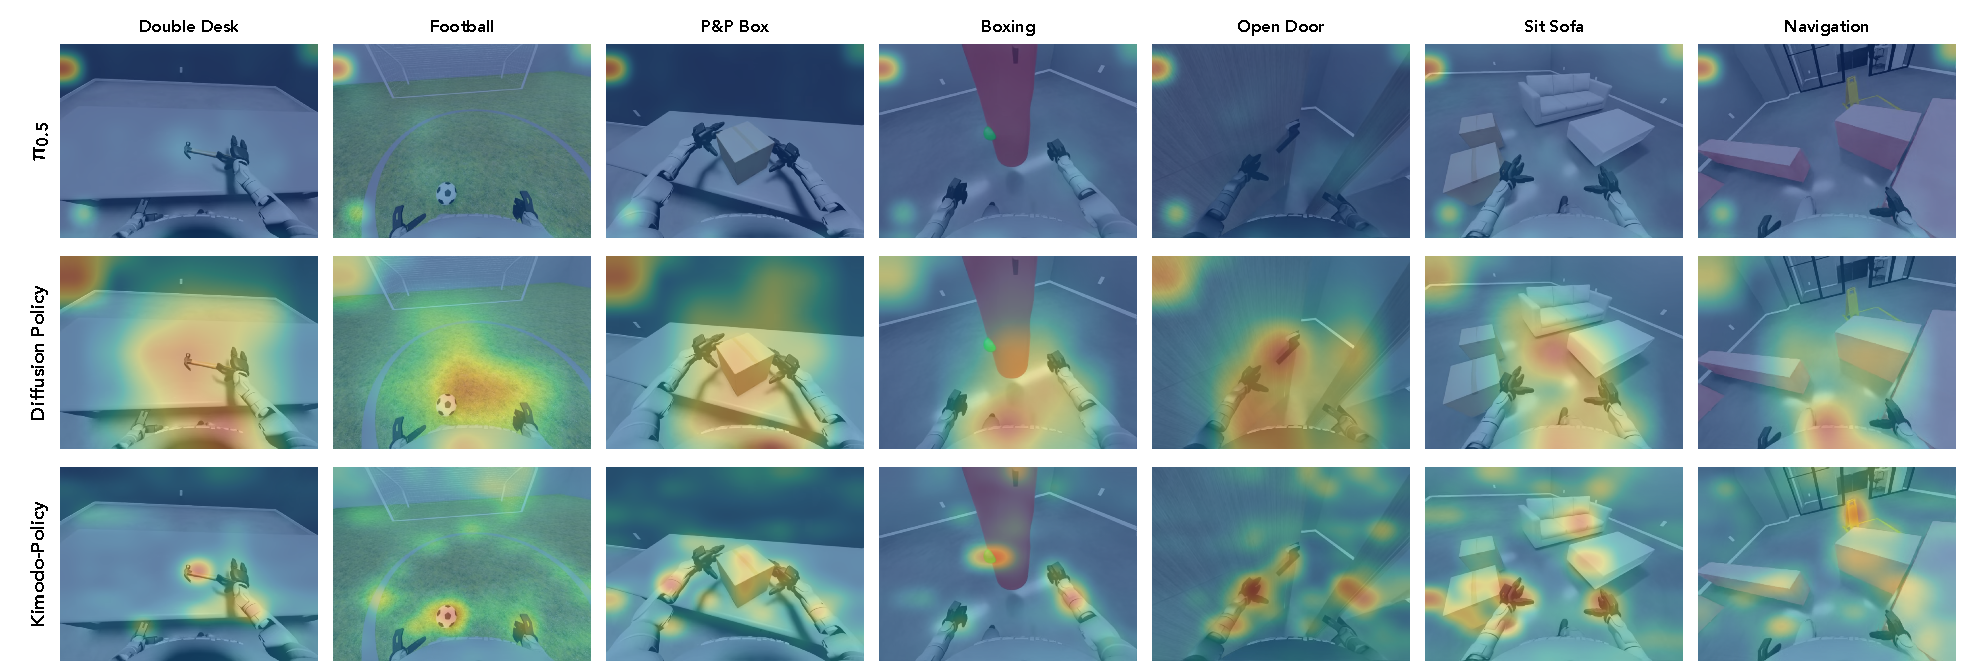
\includegraphics[width=\textwidth]{image/attention.pdf}
  \caption{\textbf{Qualitative Visual Responses Across HumanoidArena Tasks.} Columns show DoubleDesk, Football, P\&Pbox, Boxing, OpenDoor, SitSofa, and VisNavi; rows show $\pi_{0.5}$, Diffusion Policy, and Kimodo-Policy. Kimodo-Policy exhibits localized responses near interaction-relevant regions in the displayed examples.}
  \label{fig:attention}
\end{figure}

\subsection{Evaluation on the SIMPLE Benchmark}
\label{sec:exp_simple}

We next evaluate eight SIMPLE~\citep{simple} tasks covering handover, mobile manipulation, articulated-object interaction, and object pushing (Fig.~\ref{fig:simple_tasks}). An independent Kimodo-Policy$^{*}$ is fine-tuned for each task and evaluated at the L0--L2 randomization levels, which introduce progressively stronger changes in appearance, lighting, and target pose. Table~\ref{table:simple_main_results} reports ten trials per level and task, with RTC disabled for our policies. This evaluation tests whether the motion-based action generator can be adapted to different interaction requirements and remain effective under the prescribed perturbations.

\begin{figure}[H]
  \centering
  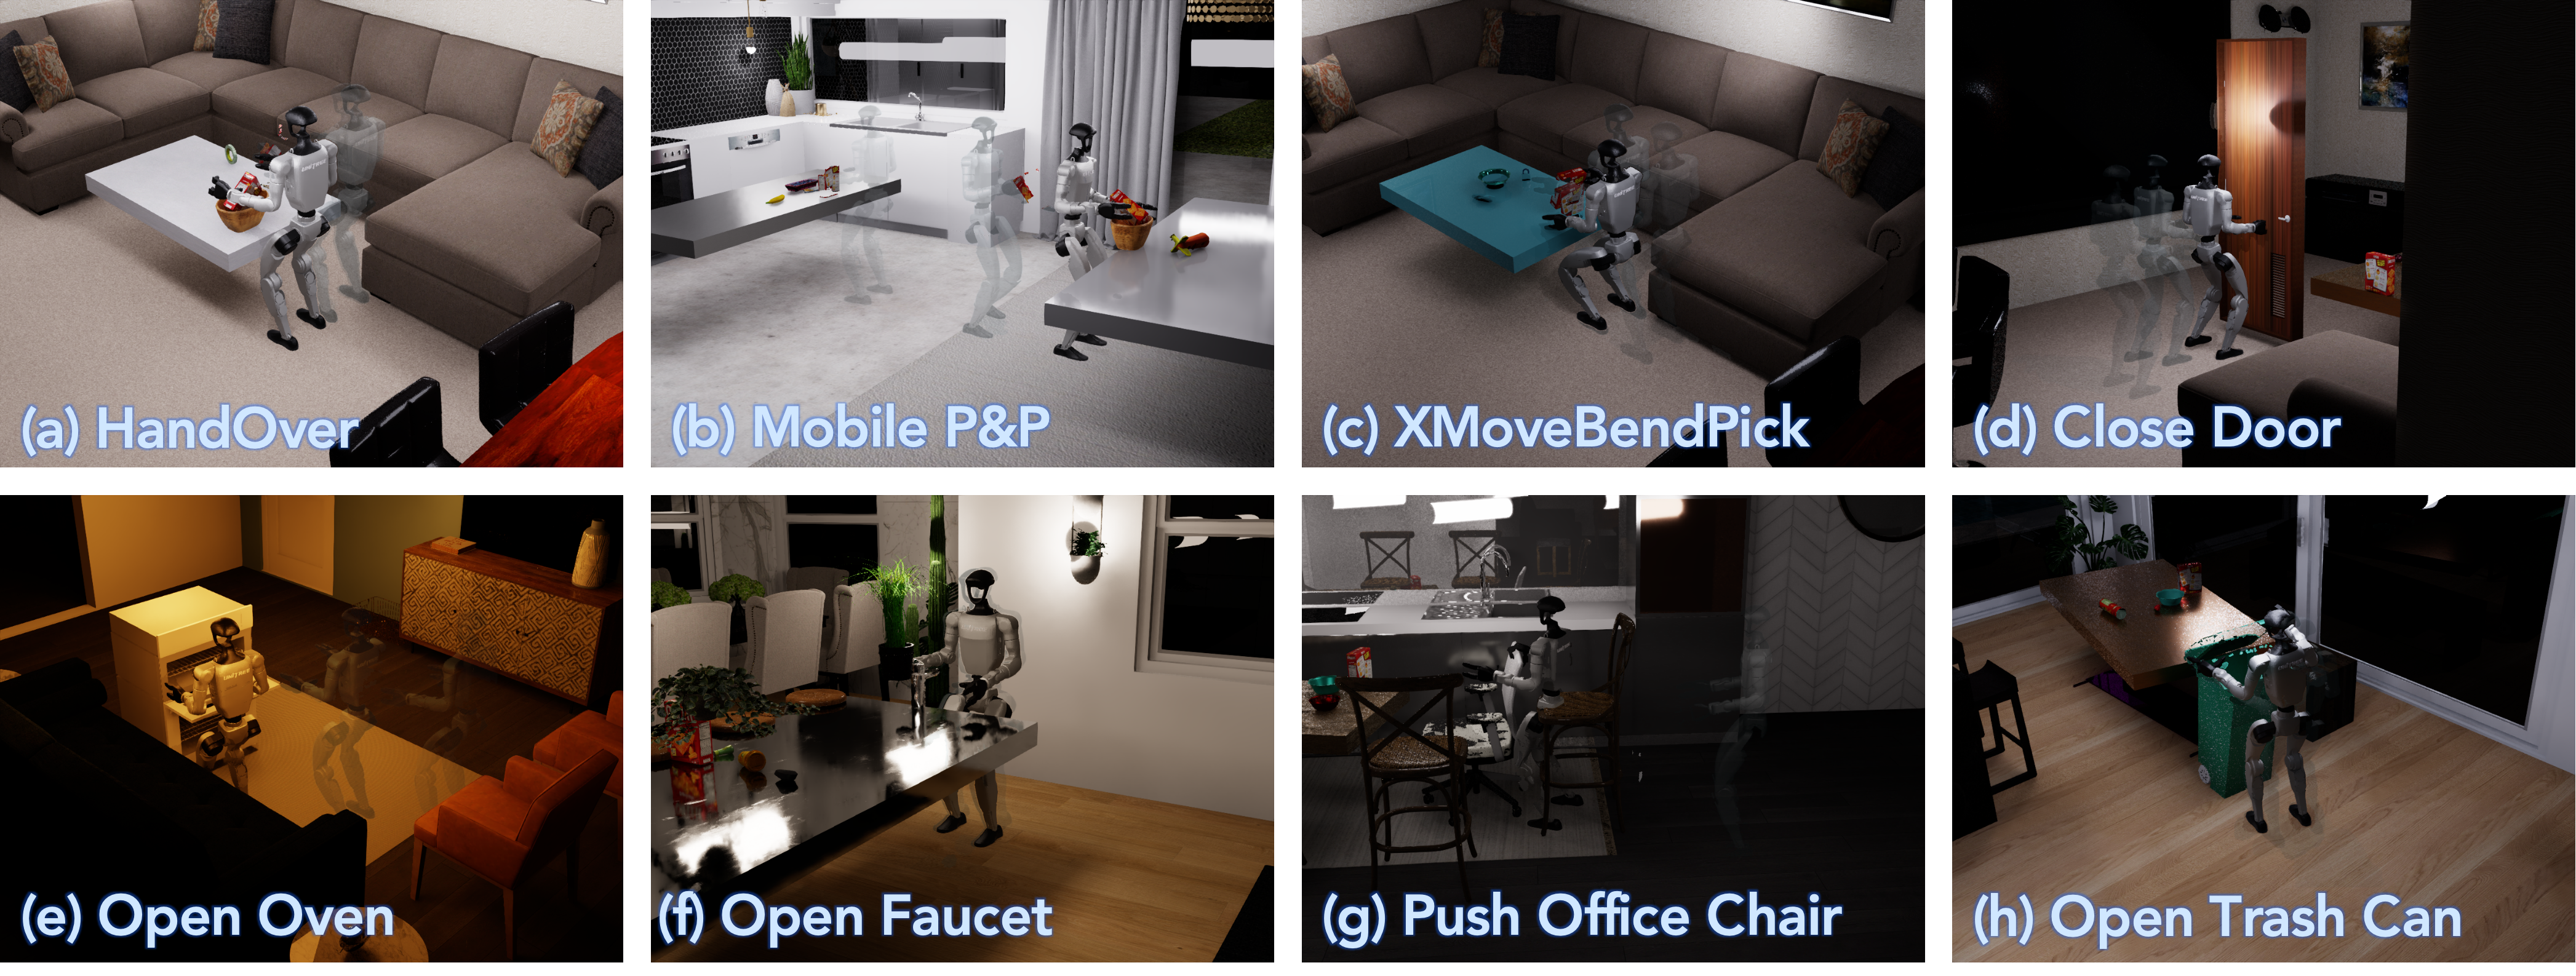
\includegraphics[width=\textwidth]{image/simple.png}
  \caption{\textbf{Evaluated SIMPLE Task Suite.} The selected tasks cover object handover and mobile pick-and-place, locomotion-integrated object pickup, articulated-object interaction, and household-object manipulation. Panels show (a) Handover, (b) Mobile P\&P, (c) XMoveBendPick, (d) CloseDoor, (e) OpenOven, (f) OpenFaucet, (g) Push Office Chair, and (h) OpenTrashCan.}
  \label{fig:simple_tasks}
\end{figure}

\begin{table}[!b]
  \caption{
    \textbf{\textit{Single-Task Results on SIMPLE.}} L0, L1, and L2 denote evaluation settings with progressively stronger visual and lighting variation and target-pose randomization, from the least perturbed setting (L0) to the most perturbed setting (L2). Each entry reports the number of successful trials at L0/L1/L2, followed in parentheses by the aggregate success rate across all three levels. Baseline results in the first three task columns are from the official SIMPLE repository; the last five $\Psi_0$ results are from Table~7 of the initial SIMPLE report~\citep{simple}. For ACT, $\pi_{0.5}$, EgoVLA, InternVLA-M1, and DP, results in the last five task columns are taken from Table~I of \citet{chen2026memorybeforegoal}. Avg is the mean success rate across all eight tasks, computed from the trial counts. Baseline rows compile results from these sources rather than a unified reevaluation; training and execution settings follow the respective reports. Rows with missing task results show a dash. Bold and underlined values mark the best and second-best aggregate success rates, respectively.
   Baselines include ACT~\citep{ACT}, DreamZero~\citep{dreamzero}, $\pi_{0.5}$~\citep{pi05}, EgoVLA~\citep{egovla}, GR00T N1.6~\citep{grootn1}, InternVLA-M1~\citep{internvla_m1}, DP~\citep{chi2023diffusionpolicy}, H-RDT~\citep{hrdt}, $\Psi_0$~\citep{psi0}.
  }
  \label{table:simple_main_results}
  \centering
  \arrayrulecolor{hclblue}
  \setlength{\tabcolsep}{0pt}
  \renewcommand{\arraystretch}{1.08}
  \fontsize{6.2}{7}\selectfont
  \newcommand{\taskheader}[1]{{\fontsize{5.55}{6.2}\selectfont\textbf{\textsc{\hspace{2.2pt}#1\hspace{2.2pt}}}}}
  \newcommand{\resultentry}[2]{{\fontsize{5.2}{6}\selectfont\hspace{2.2pt}#1\;(#2)\hspace{2.2pt}}}
  \newcommand{\bestentry}[2]{{\fontsize{5.2}{6}\selectfont\textbf{\hspace{2.2pt}#1\;(#2)\hspace{2.2pt}}}}
  \newcommand{\secondentry}[2]{{\fontsize{5.2}{6}\selectfont\hspace{2.2pt}\underline{#1\;(#2)}\hspace{2.2pt}}}

  \newcommand{\avgentry}[1]{{\fontsize{5.2}{6}\selectfont\hspace{2.2pt}#1\hspace{2.2pt}}}
  \begin{adjustbox}{width=\textwidth}
  \begin{tabular}{@{}c*{9}{c}@{}}
    \toprule
    {\fontsize{5.55}{6.2}\selectfont\textbf{Method}}
    & \taskheader{Handover}
    & \taskheader{Mobile P\&P}
    & \taskheader{XMoveBendPick}
    & \taskheader{CloseDoor}
    & \taskheader{OpenOven}
    & \taskheader{OpenFaucet}
    & \taskheader{Push Office Chair}
    & \taskheader{OpenTrashCan}
    & \taskheader{Avg ($\uparrow$)} \\
    \midrule

    ACT
    & \resultentry{4/4/6}{47\%}
    & \secondentry{6/5/7}{60\%}
    & \resultentry{6/8/8}{73\%}
    & \bestentry{10/10/10}{100\%} & \resultentry{1/0/1}{7\%} & \resultentry{0/0/1}{3\%} & \secondentry{9/10/10}{97\%} & \resultentry{4/4/7}{50\%}
    & \avgentry{54.58\%} \\

    DreamZero
    & \secondentry{7/8/9}{80\%}
    & \resultentry{5/3/3}{37\%}
    & \resultentry{0/0/1}{3\%}
    & - & - & - & - & -
    & \avgentry{-} \\

    $\pi_{0.5}$
    & \resultentry{5/4/5}{47\%}
    & \resultentry{3/3/3}{30\%}
    & \resultentry{0/0/0}{0\%}
    & \secondentry{10/10/9}{97\%} & \resultentry{4/3/6}{43\%} & \resultentry{4/2/0}{20\%} & \resultentry{10/10/6}{87\%} & \resultentry{7/6/5}{60\%}
    & \avgentry{47.92\%} \\

    EgoVLA
    & \resultentry{0/4/3}{23\%}
    & \resultentry{0/0/0}{0\%}
    & \resultentry{3/5/4}{40\%}
    & \resultentry{10/8/10}{93\%} & \resultentry{5/8/2}{50\%} & \resultentry{0/0/0}{0\%} & \secondentry{10/9/10}{97\%} & \resultentry{3/5/4}{40\%}
    & \avgentry{42.92\%} \\

    GR00T N1.6
    & \resultentry{1/3/3}{23\%}
    & \resultentry{0/0/0}{0\%}
    & \resultentry{4/4/1}{30\%}
    & - & - & - & - & -
    & \avgentry{-} \\

    InternVLA-M1
    & \resultentry{0/0/0}{0\%}
    & \resultentry{0/0/0}{0\%}
    & \resultentry{3/5/7}{50\%}
    & \resultentry{0/0/0}{0\%} & \bestentry{8/6/8}{73\%} & \resultentry{0/0/0}{0\%} & \resultentry{2/3/1}{20\%} & \resultentry{0/0/0}{0\%}
    & \avgentry{17.92\%} \\

    DP
    & \resultentry{3/2/4}{30\%}
    & \resultentry{4/0/0}{13\%}
    & \resultentry{0/0/0}{0\%}
    & \bestentry{10/10/10}{100\%} & \resultentry{0/0/0}{0\%} & \secondentry{2/3/6}{37\%} & \resultentry{10/6/8}{80\%} & \resultentry{4/7/7}{60\%}
    & \avgentry{40.00\%} \\

    H-RDT
    & \resultentry{0/1/0}{3\%}
    & \resultentry{0/0/0}{0\%}
    & \resultentry{0/0/0}{0\%}
    & - & - & - & - & -
    & \avgentry{-} \\

    $\Psi_0$
    & \secondentry{7/7/10}{80\%}
    & \secondentry{7/5/6}{60\%}
    & \bestentry{10/9/9}{93\%}
    & \bestentry{10/10/10}{100\%}
    & \resultentry{7/5/4}{53\%}
    & \resultentry{3/3/4}{33\%}
    & \bestentry{10/10/10}{100\%}
    & \bestentry{7/9/9}{83\%}
    & \avgentry{\underline{75.42\%}} \\

    \rowcolor{hclbrown!15!white}
    \texttt{Ours}$^{*}$
    & \bestentry{9/8/8}{83\%}
    & \bestentry{9/8/4}{70.0\%}
    & \secondentry{10/7/7}{80\%}
    & \bestentry{10/10/10}{100\%}
    & \secondentry{8/4/5}{57\%}
    & \bestentry{5/6/5}{53\%}
    & \bestentry{10/10/10}{100\%}
    & \secondentry{9/4/6}{63\%}
    & \avgentry{\textbf{75.83\%}} \\

    \bottomrule
  \end{tabular}
  \end{adjustbox}
\end{table}


\textbf{Single-task results.} Kimodo-Policy$^{*}$ achieves 75.83\% mean SR across the eight tasks, compared with 75.42\% for $\Psi_0$~\citep{psi0}, the strongest baseline with complete task coverage. These values correspond to 182 and 181 successful trials out of 240, respectively. Baseline results are compiled from the official SIMPLE release and a subsequent evaluation~\citep{simple,chen2026memorybeforegoal}, as specified in the table caption; they are not a unified reevaluation under our training and execution pipeline. The aggregate performance is therefore comparable, with a small numerical advantage for Kimodo-Policy$^{*}$. Kimodo-Policy$^{*}$ attains the best or joint-best SR on five tasks. It leads on Handover (25/30 successes), Mobile P\&P (21/30), and OpenFaucet (16/30), compared with the strongest baseline counts of 24/30, 18/30, and 11/30, respectively. It also achieves 30/30 on both CloseDoor and Push Office Chair, tying the best reported results. It ranks second on the remaining three tasks: XMoveBendPick (24/30 versus 28/30 for $\Psi_0$), OpenOven (17/30 versus 22/30 for InternVLA-M1~\citep{internvla_m1}), and OpenTrashCan (19/30 versus 25/30 for $\Psi_0$). This distribution demonstrates broad applicability of the motion-based policy while identifying interaction types for which other approaches remain stronger. Averaged across the eight tasks, Kimodo-Policy$^{*}$ achieves 87.50\%, 71.25\%, and 68.75\% SR at L0, L1, and L2, respectively. Performance remains perfect on CloseDoor and Push Office Chair, whereas Mobile P\&P declines from 9/10 at L0 to 4/10 at L2. The adapted policy therefore remains sensitive to perceptual and geometric variation despite its inherited motion prior. Together, these results support competitive task performance while identifying robustness as an important remaining challenge.

\subsection{Evaluation on the Real-World Humanoid Robot}
\label{sec:exp_real}

We deploy Kimodo-Policy on a physical humanoid to evaluate the complete perception--generation--tracking pipeline beyond simulation. The eight tasks require different combinations of locomotion, posture adjustment, single- and dual-arm coordination, and object interaction (Fig.~\ref{fig:real_world}). Each policy is evaluated for ten trials per task. Deployment follows Sec.~\ref{sec:setup_posttraining}, including RTC for Kimodo-Policy. Both Kimodo-Policy variants retain the pretrained motion backbone and differ in whether the trainable modules undergo policy pretraining before task-specific fine-tuning.

\begin{figure}[H]
  \centering
  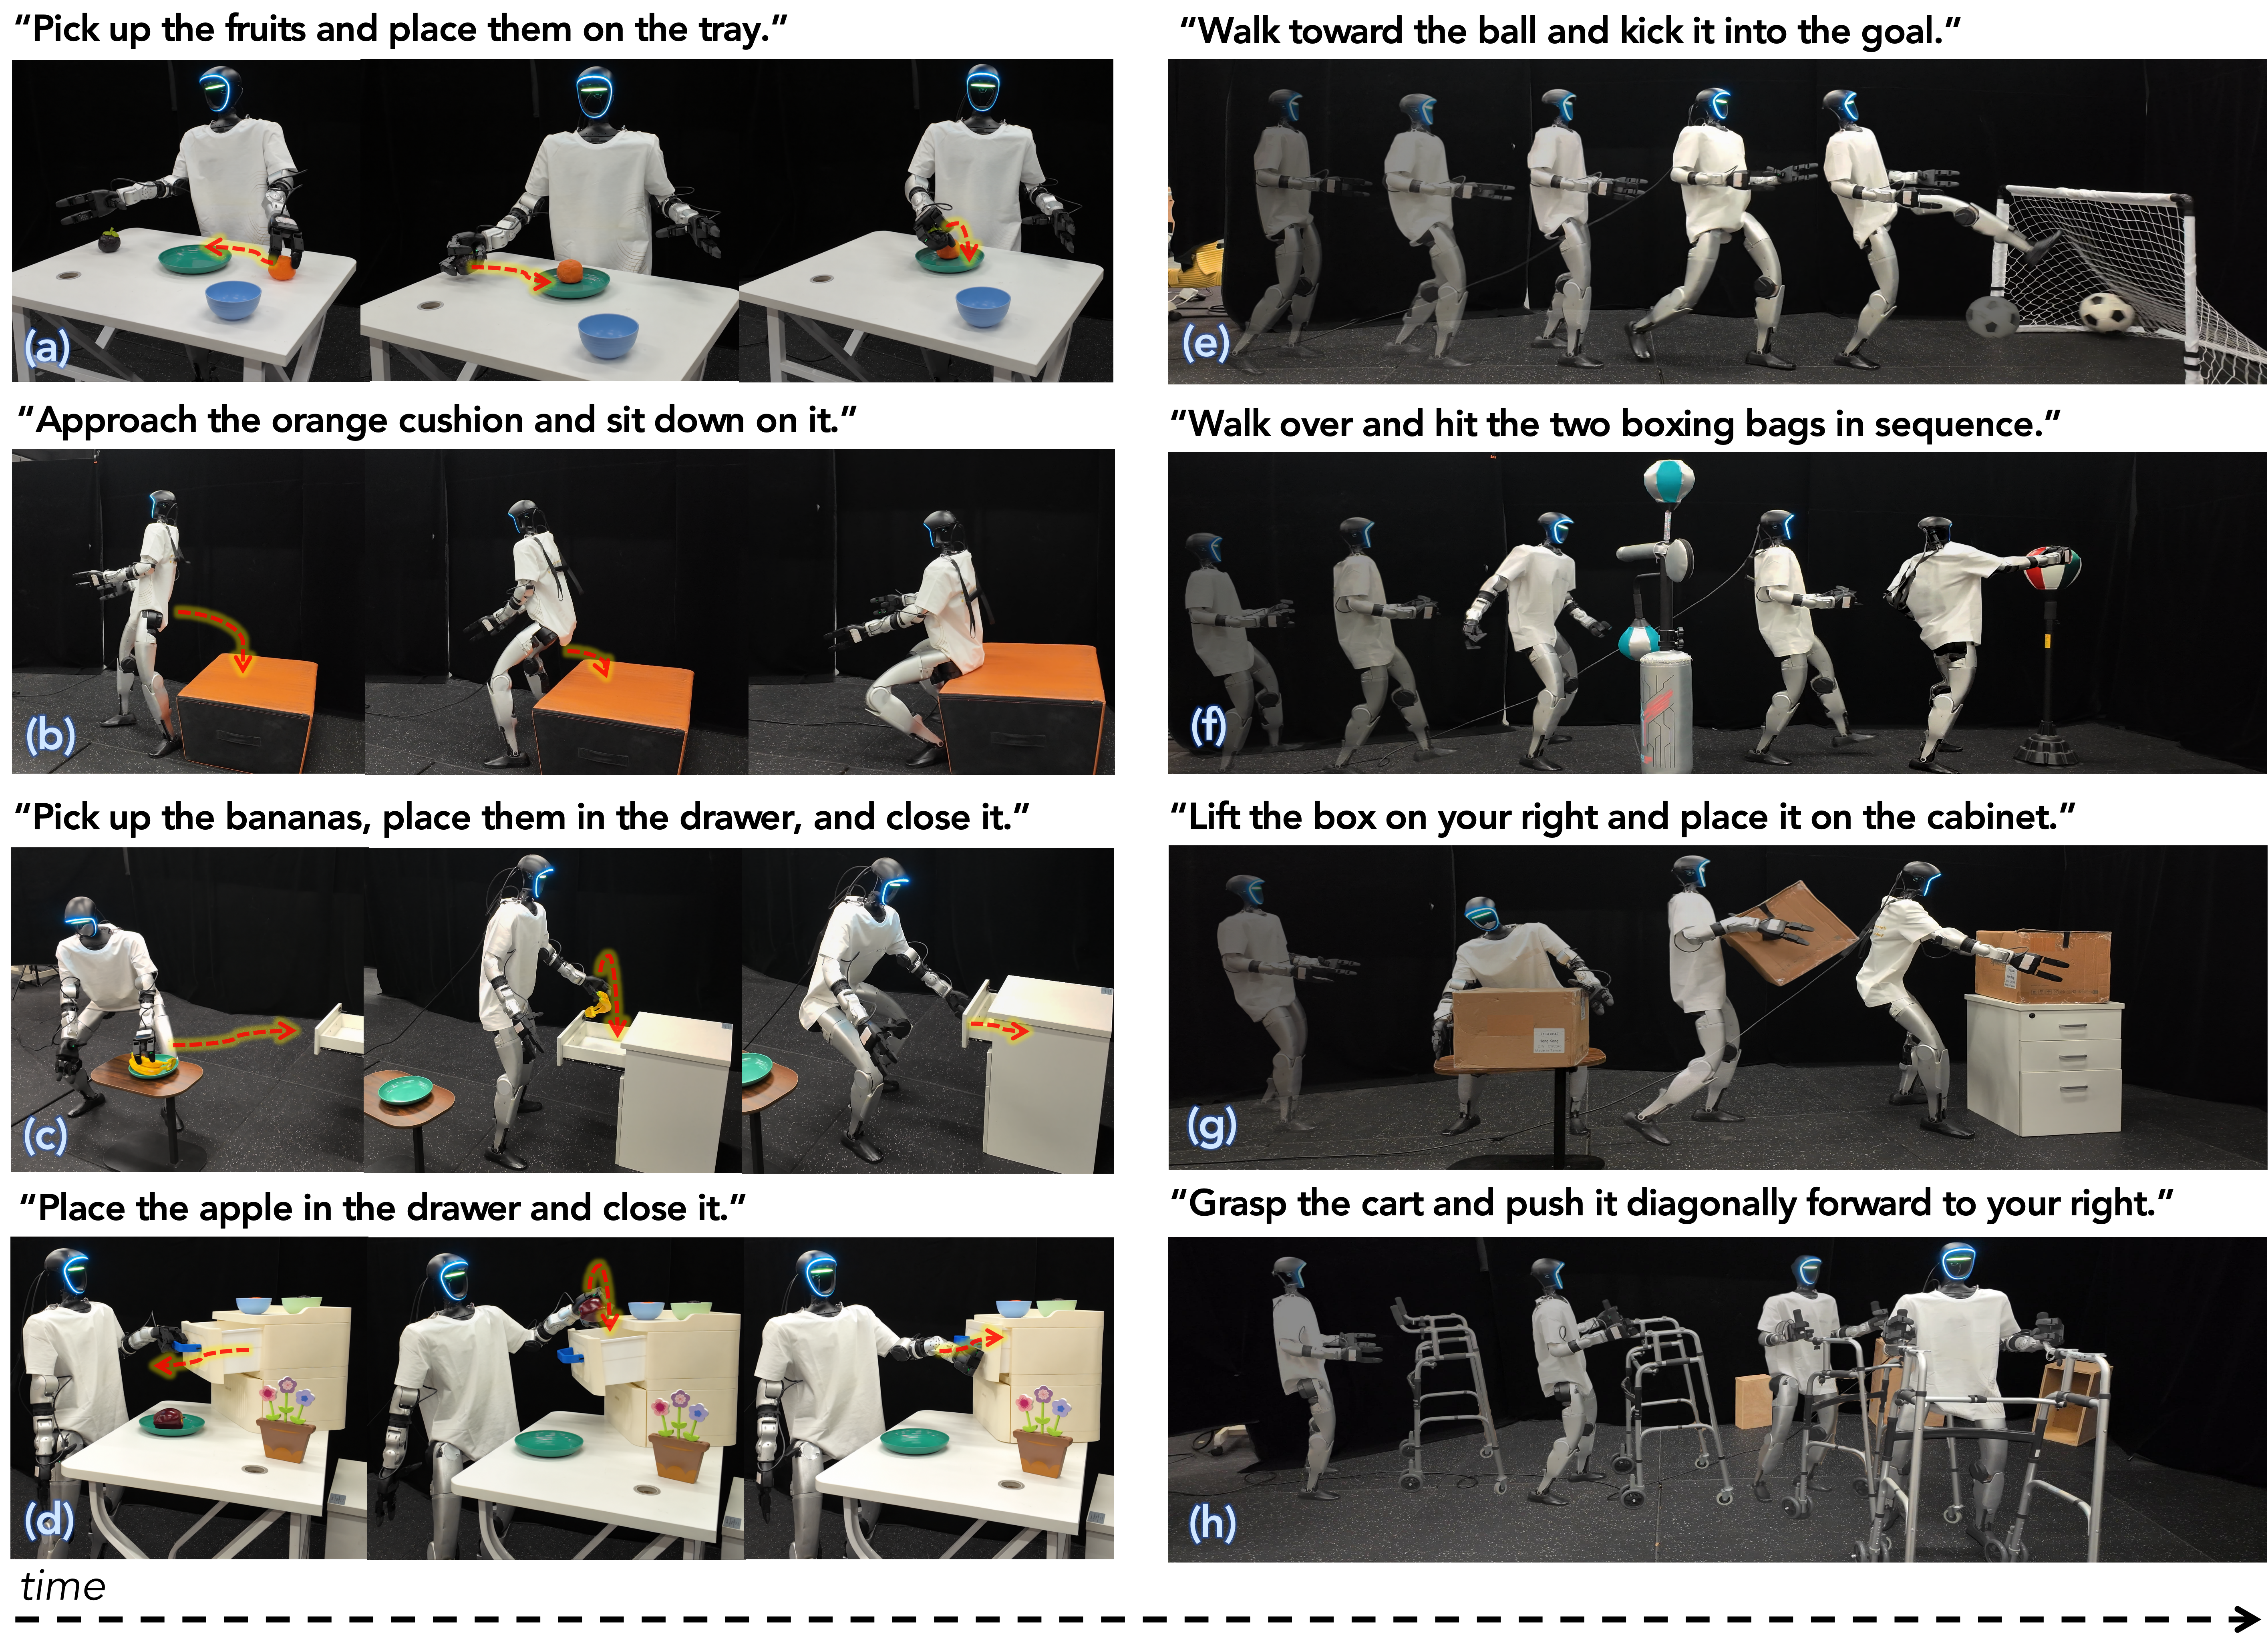
\includegraphics[width=\textwidth]{image/real_world.png}
  \caption{\textbf{Examples of Real-World Humanoid Manipulation.} The image shows representative interaction scenarios involving articulated objects, object transport, and coordinated whole-body motion.}
  \label{fig:real_world}
\end{figure}

\textbf{Real-world results.} As shown in Fig.~\ref{fig:real_world_success_rates}, Kimodo-Policy without additional policy pretraining achieves 45\% mean SR, compared with approximately 31\% for GR00T N1.6~\citep{grootn1} and 35\% for $\Psi_0$. Policy pretraining increases the mean to 60\%, corresponding to 48 successful trials out of 80 and a 15-percentage-point gain over direct fine-tuning. The pretrained variant improves on seven tasks and matches the directly fine-tuned variant on Cart Pushing (60\%). Its highest SRs are 90\% on Punching Bag, 80\% on Cushion Sitting, and 70\% on Dual-Arm PNP. Improvements are largest on Football Scoring (20\% to 50\%), followed by Dual-Arm PNP, Banana Cabinet, and Box Carrying (20 percentage points each). These results provide initial evidence for KAMs on a physical robot. A motion generator conditioned on current observations and coupled to a whole-body tracker supports the evaluated locomotion and manipulation tasks. Because the motion backbone is shared by both variants, their performance difference supports the complementary value of robot-interaction pretraining for adapting the conditioning modules and hand head. The baseline comparison evaluates the deployed systems as a whole; the effect of RTC is not separately ablated. With ten trials per task, the reported rates characterize performance on this evaluation set rather than establish deployment reliability across unrestricted environments.

\begin{figure}[H]
  \centering
  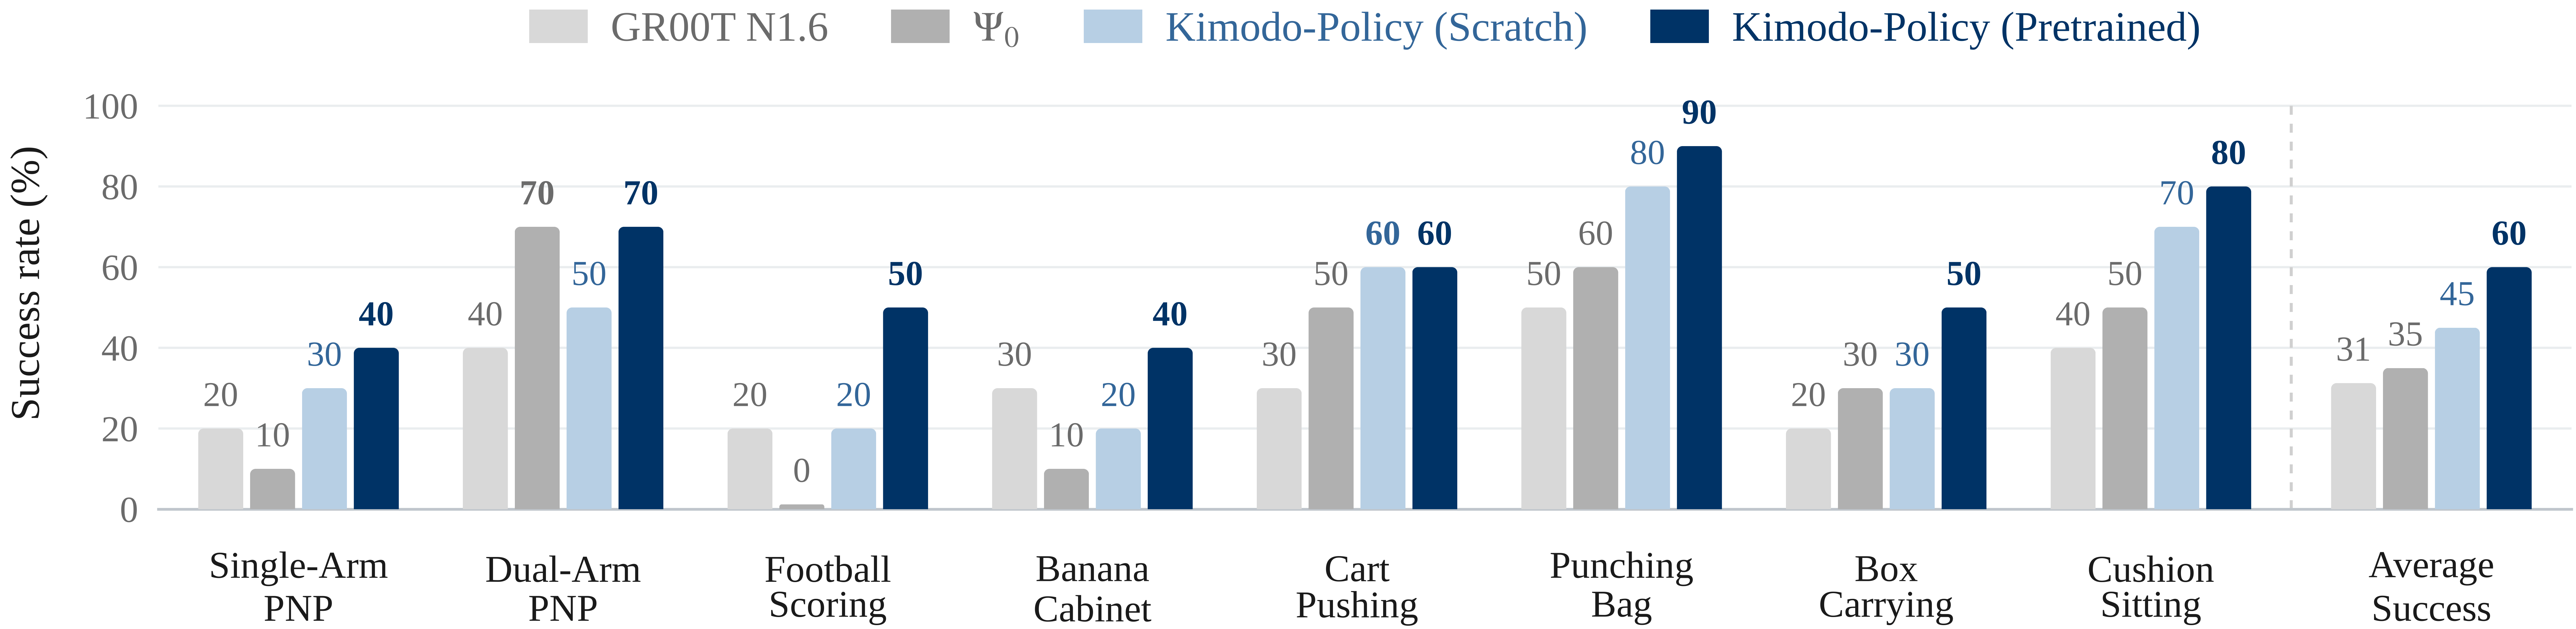
\includegraphics[width=\textwidth]{image/real_world_success_rates.png}
  \caption{\textbf{Real-World Task Success.} Success rates for GR00T N1.6, $\Psi_0$, and Kimodo-Policy with and without additional robot-interaction policy pretraining. Both Kimodo-Policy variants retain the pretrained motion backbone. Each task is evaluated for ten trials; the rightmost group reports the mean across eight tasks. The plot label \emph{Scratch} denotes the variant without additional policy pretraining, while \emph{Pretrained} denotes the variant with it.}
  \label{fig:real_world_success_rates}
\end{figure}

\subsection{How Does the Choice of Motion Prior Affect Downstream Control?}
\label{sec:exp_t2m}

A central implication of KAMs is that the action-generating backbone should matter beyond its parameter count. We examine this by substituting two pretrained Kimodo-G1 variants~\citep{kimodo} while retaining the policy architecture, adaptation procedure, and HumanoidArena evaluation protocol. Both backbones contain 282M parameters. The released SEED-v1 and RP-v1 checkpoints specify motion corpora of 288 h and approximately 560 h, respectively, with 90\%/10\% train/test splits. This comparison evaluates the downstream consequences of selecting different motion priors at matched backbone capacity.

\begin{table}[H]
  \caption{
    \textbf{\textit{Effect of the T2M backbone on Kimodo-Policy.}} We compare two same-size Kimodo-G1 backbones using the same adaptation protocol. Data scales include the training and test splits; results are mean $\pm$ standard deviation over three seeds.}
  \label{tab:t2m_dependency}
  \centering
  \arrayrulecolor{hclblue}
  \begin{adjustbox}{max width=\textwidth}
  \setlength{\tabcolsep}{3.8pt}
  \renewcommand{\arraystretch}{1.08}

  \begin{tabular}{cccccc|ccccc}
  \toprule
  \multirow{2}{*}{\textbf{Base Model}} &
  \multirow{2}{*}{\textbf{Model Size}} &
  \multirow{2}{*}{\textbf{Data Scale}} &
  \multicolumn{3}{c|}{\textbf{Human--Object Interaction}} &
  \multicolumn{4}{c}{\textbf{Human--Scene Interaction}} &
  \multirow{2}{*}{\textbf{Overall~($\uparrow$)}} \\
  \cmidrule(lr){4-6}
  \cmidrule(lr){7-10}

  & & &
  \textbf{\textsc{Football}} &
  \textbf{\textsc{DoubleDesk}} &
  \textbf{\textsc{P\&Pbox}} &
  \textbf{\textsc{OpenDoor}} &
  \textbf{\textsc{SitSofa}} &
  \textbf{\textsc{Boxing}} &
  \textbf{\textsc{VisNavi}} \\
  \midrule

  \texttt{Kimodo-G1-SEED-v1}
  & 282\,M
  & 288\,h
  & \textbf{50.00$\pm$16.33\%}
  & \underline{33.33$\pm$15.46\%}
  & \underline{75.00$\pm$10.80\%}
  & \underline{60.00$\pm$4.08\%}
  & \underline{90.00$\pm$4.08\%}
  & \textbf{71.67$\pm$8.50\%}
  & \textbf{70.00$\pm$18.71\%}
  & \underline{64.29\%} \\

  \rowcolor{hclbrown!8!white}
  \texttt{Kimodo-G1-RP-v1}
  & 282\,M
  & 700\,h
  & \underline{35.0$\pm$7.1\%}
  & \textbf{40.0$\pm$0.0\%}
  & \textbf{80.0$\pm$4.1\%}
  & \textbf{93.3$\pm$6.2\%}
  & \textbf{96.7$\pm$4.7\%}
  & \underline{66.7$\pm$4.7\%}
  & \underline{61.7$\pm$6.2\%}
  & \textbf{67.63\%} \\

  \bottomrule
  \end{tabular}
  \end{adjustbox}
\end{table}


\textbf{Motion-prior transfer results.} Table~\ref{tab:t2m_dependency} reports an overall SR of 64.29\% for SEED-v1 and 67.63\% for RP-v1, a difference of 3.34 percentage points. The gains are task dependent: RP-v1 improves DoubleDesk, P\&Pbox, OpenDoor, and SitSofa, with the largest increase on OpenDoor (60.0\% to 93.3\%). Conversely, Football declines from 50.0\% to 35.0\%, Boxing from 71.67\% to 66.7\%, and VisNavi from 70.0\% to 61.7\%. The overall improvement is thus driven primarily by the net gain on scene-interaction tasks, rather than a uniform improvement across behaviors. The fixed parameter budget makes this result relevant to the KAM premise: the choice of pretrained motion generator affects downstream control even when policy capacity is unchanged. However, the two corpora differ in both size and content, and Table~\ref{tab:t2m_dependency} does not report an independent motion-generation quality metric. The comparison therefore supports the importance of the inherited motion prior, but does not establish a monotonic relationship between T2M quality and control performance or isolate motion-data scale as the cause of the gain.

\subsection{Scaling Robot-Interaction Data and Trainable Policy Capacity}
\label{sec:exp_scaling}

We examine two ways of strengthening the adaptation of a fixed motion backbone: increasing robot-interaction pretraining data and increasing trainable policy capacity. The data sweep holds the policy architecture and downstream seven-task adaptation protocol fixed. The capacity sweep retains the same pretrained motion backbone, downstream data, and optimization protocol while varying the trainable parameter budget. RTC is disabled throughout. These experiments concern policy adaptation around the motion prior, rather than scaling the motion generator itself.

\begin{figure}[H]
  \centering
  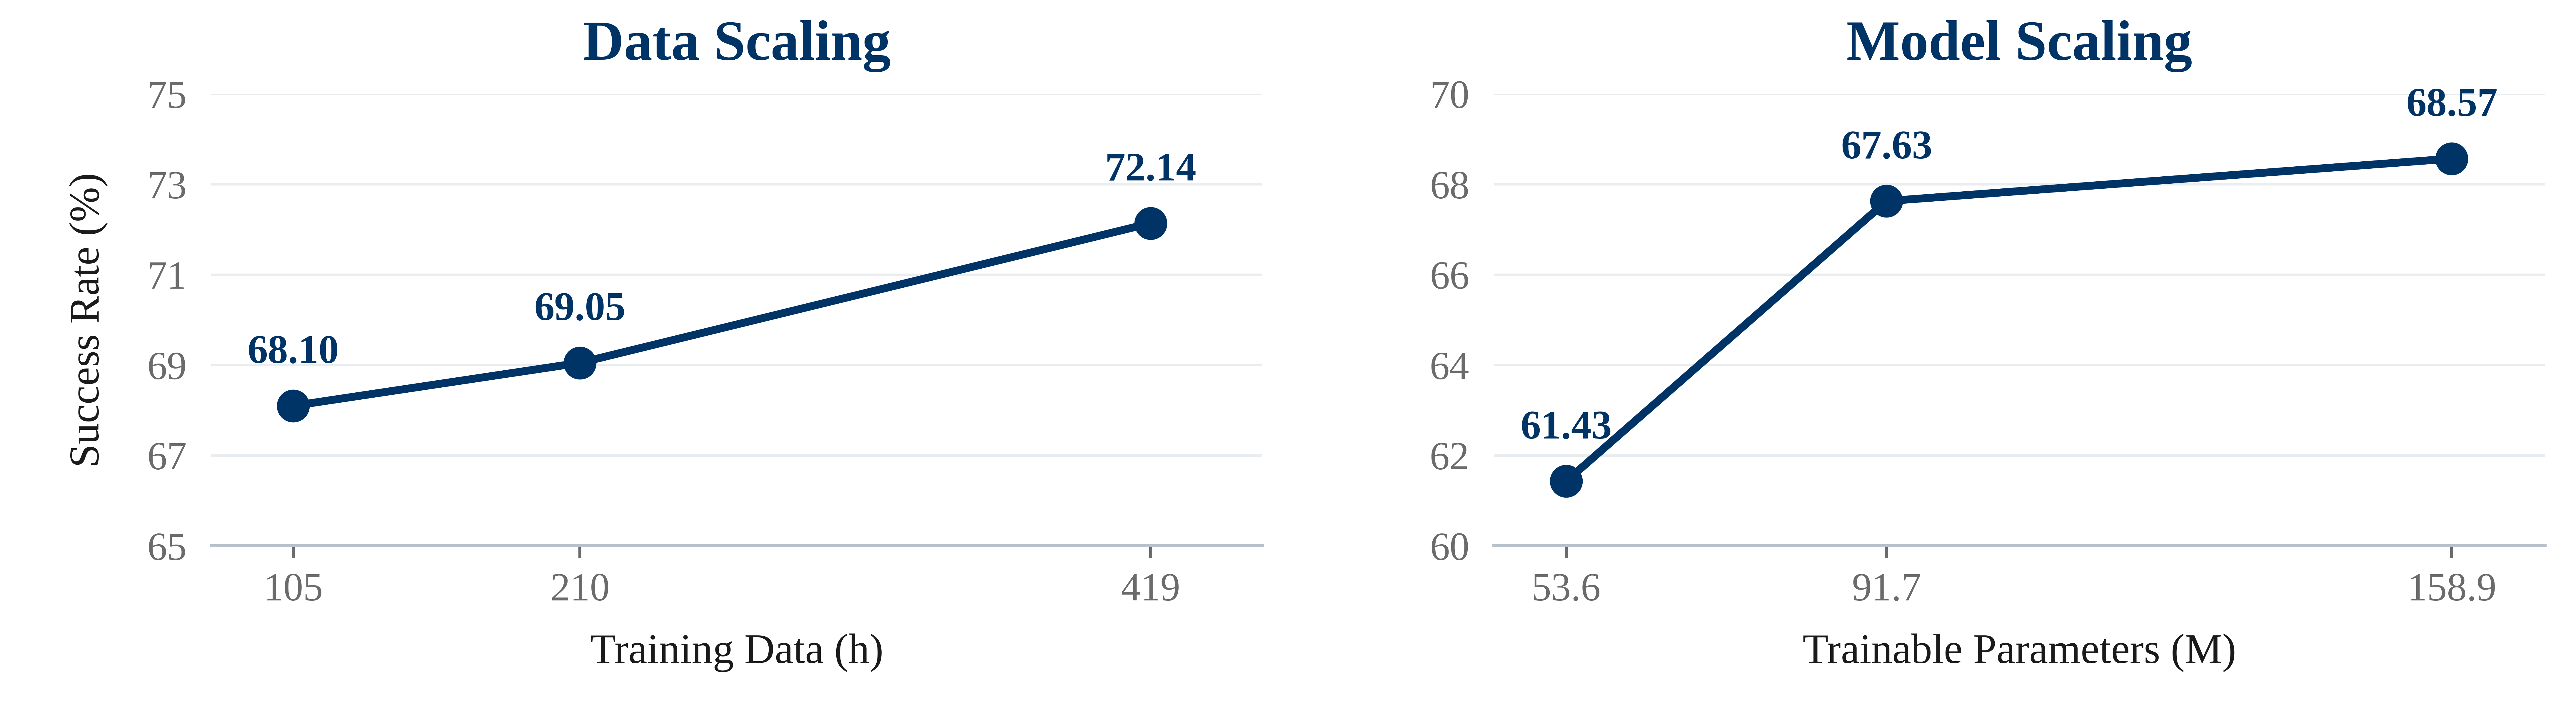
\includegraphics[width=\textwidth]{image/scaling_analysis.png}
  \caption{\textbf{Scaling Policy Adaptation Around a Fixed Motion Backbone.} Overall success on the seven HumanoidArena tasks as a function of robot-interaction policy-pretraining data (left) and trainable policy parameters (right). The motion backbone is held fixed in both sweeps. Each panel follows its respective controlled adaptation setting and should not be interpreted as a joint data--capacity sweep.}
  \label{fig:scaling_analysis}
\end{figure}

\textbf{Scaling results.} Figure~\ref{fig:scaling_analysis} shows that overall SR increases from 68.10\% with 105 h of policy-pretraining data to 69.05\% with 210 h and 72.14\% with 419 h, a total gain of 4.04 percentage points. With the motion backbone fixed, these gains show that additional interaction demonstrations can improve the learned conditioning and hand-control components. This complements the role of motion pretraining in the KAM formulation: an inherited movement repertoire provides a foundation, while robot-interaction data adapt its use to observations and task objectives. The observed increase is consistent across the three evaluated data budgets, although it does not by itself establish a scaling law or predict gains beyond this range. For trainable policy capacity, increasing the trainable parameter count from 53.6M to 91.7M raises overall SR from 61.43\% to 67.63\%; a further increase to 158.9M yields 68.57\%. The total improvement is 7.14 percentage points, with a larger gain in the first increment (6.20 points) than in the second (0.94 points). Thus, downstream performance benefits from additional adaptation capacity within the tested range, with diminishing observed returns. The 91.7M configuration used in the main policy remains within 0.94 points of the largest evaluated configuration while using approximately 42\% fewer trainable parameters. This comparison supports the selected trainable parameter budget; inference efficiency is not measured in this sweep.

\begin{figure}[!b]
  \centering
  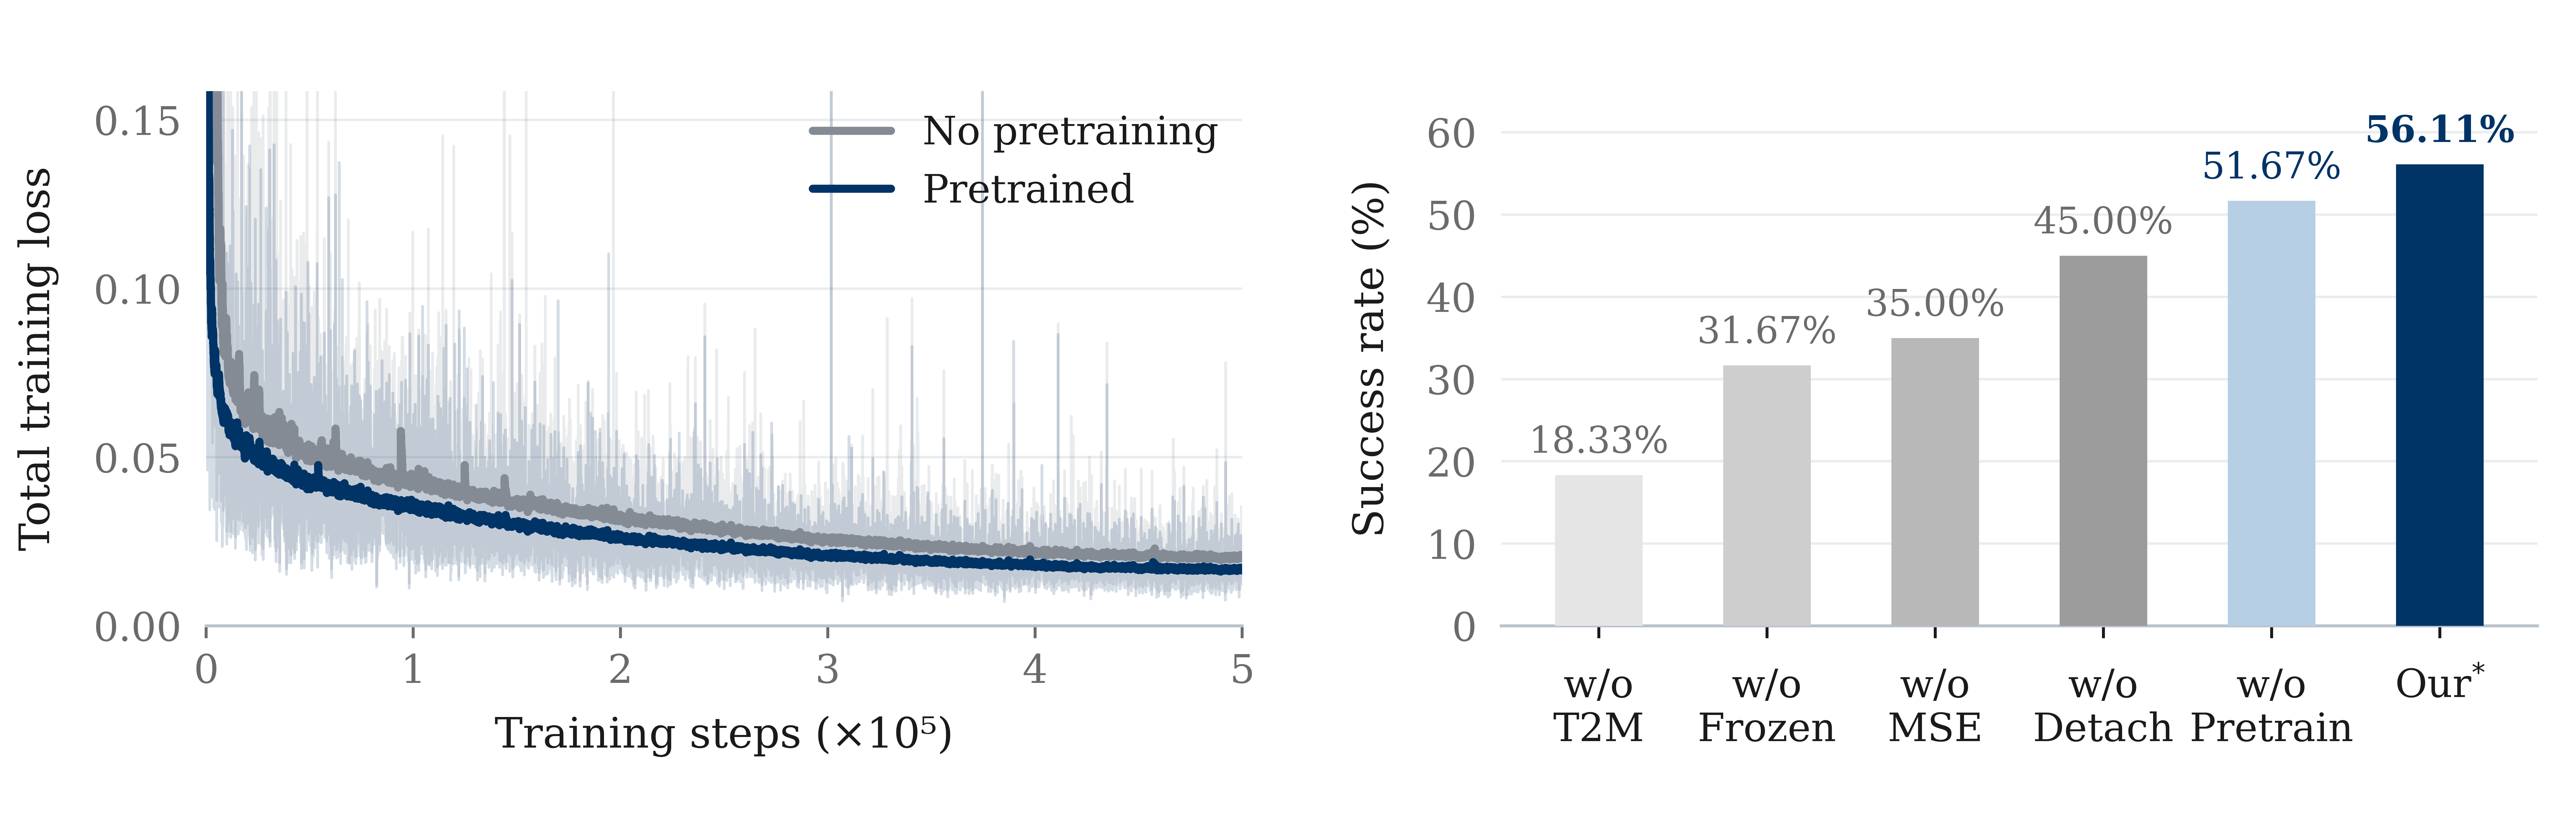
\includegraphics[width=\textwidth]{image/training_loss_comparison.png}
  \caption{\textbf{Policy Adaptation Dynamics and Ablations.} Left: downstream training-loss trajectories with and without additional policy pretraining; both variants retain the pretrained motion backbone. Right: mean success across DoubleDesk, Football, and P\&Pbox after joint seven-task training. Gray bars show independent ablations of the T2M backbone (w/o T2M), backbone freezing (w/o Frozen), the MSE objective (w/o MSE), and root--body gradient detachment (w/o Detach), each relative to the reference without policy pretraining (light blue). Dark blue shows the result with additional policy pretraining.}
  \label{fig:training_loss_comparison}
\end{figure}

\begingroup
\titleformat{\subsection}
  {\normalfont\fontsize{14pt}{17pt}\selectfont\bfseries\color{black}}
  {\thesubsection}{0.55em}{}
\subsection{Ablation Study}
\label{sec:exp_ablation}
\color{black}

We examine the motion backbone, backbone freezing, prediction objective, root--body gradient decoupling, and additional policy pretraining. All variants are trained in the joint seven-task HumanoidArena setting; the ablation metric in Fig.~\ref{fig:training_loss_comparison} averages SR over the three HOI tasks, DoubleDesk, Football, and P\&Pbox. The reference without additional policy pretraining achieves 51.67\%. Each component ablation is compared with this reference, while the effect of policy pretraining is evaluated separately. These three-task averages should be distinguished from the seven-task overall scores in Table~\ref{tab:arena_multi_task}.

\textbf{Ablation results.} The variant labeled w/o T2M achieves 18.33\% SR, 33.34 percentage points below the reference. This is the largest reduction among the evaluated component ablations and supports the importance of the motion-backbone component in this instantiation. Unfreezing the backbone reduces SR to 31.67\%, a 20.00-point drop. Under the evaluated adaptation protocol, retaining the pretrained generator and learning its conditioning through separate trainable branches is therefore more effective than updating the backbone jointly. For the prediction objective, replacing MSE with the original Kimodo motion objective yields 35.00\% SR, 16.67 percentage points below the reference. This favors the direct prediction objective for the evaluated downstream adaptation setting. Separately, removing root--body gradient detachment yields 45.00\%, a reduction of 6.67 points. Detachment preserves the forward dependence of body generation on root predictions while preventing body-stage supervision from updating the root ControlNet. Its benefit shows that forward coordination and coupled optimization need not be implemented through the same gradient pathways. These ablations support the selected objective and gradient boundaries for adapting the hierarchical generator. Finally, additional policy pretraining raises mean SR from 51.67\% to 56.11\%, a gain of 4.44 percentage points. Figure~\ref{fig:training_loss_comparison} also shows generally lower downstream training loss for the pretrained initialization. Since both variants retain the same pretrained motion backbone, the performance gain supports the complementary contribution of learning observation-conditioned interaction before downstream fine-tuning. Taken together, the ablations support a central design principle of this KAM instantiation: preserve a pretrained motion generator, learn how to condition it for interaction, and use task-appropriate objectives and gradient boundaries during adaptation.

\endgroup
